%! app: decidable languages, undecidable languages
%! outcome: Classify language, Find example languages, Define decision problem, Classify decision problem
    
\begin{center}
    \begin{tabular}{|lcl|}
    \hline
    \multicolumn{3}{|l|}{{\bf  Acceptance problem} } \\
    & & \\
    \ldots for DFA & $A_{DFA}$ & $\{ \langle B,w \rangle \mid  \text{$B$ is a  DFA that accepts input 
    string $w$}\}$ \\
    \ldots for NFA & $A_{NFA}$ & $\{ \langle B,w \rangle \mid  \text{$B$ is a  NFA that accepts input 
    string $w$}\}$ \\
    \ldots for regular expressions & $A_{REX}$ & $\{ \langle R,w \rangle \mid  \text{$R$ is a  regular
    expression that generates input string $w$}\}$ \\
    \ldots for CFG & $A_{CFG}$ & $\{ \langle G,w \rangle \mid  \text{$G$ is a context-free grammar 
    that generates input string $w$}\}$ \\
    \ldots for PDA & $A_{PDA}$ & $\{ \langle B,w \rangle \mid  \text{$B$ is a PDA that accepts input string $w$}\}$ \\
    & & \\
    & & \\
    \hline
    \end{tabular}
\end{center}

\newpage
\begin{center}
\begin{tabular}{|lcl|}
\hline
\multicolumn{3}{|l|}{{\bf  Acceptance problem} } \\
for Turing  machines  & $A_{TM}$ & $\{ \langle M,w \rangle \mid  \text{$M$ is a Turing machine that accepts input 
string $w$}\}$ \\
\hline
\multicolumn{3}{|l|}{{\bf Language emptiness  testing} } \\
 for Turing machines & $E_{TM}$ & $\{ \langle M \rangle \mid  \text{$M$ is a Turing machine and  $L(M) = \emptyset$\}}$ \\
\hline
\multicolumn{3}{|l|}{{\bf Language equality testing} } \\
 for Turing machines& $EQ_{TM}$ & $\{ \langle  M_1, M_2 \rangle \mid  \text{$M_1$ and $M_2$ are Turing machines and  
 $L(M_1) =L(M_2)$\}}$\\
\hline
Sipser Section 4.1 &&\\
\hline
\end{tabular}
\end{center}

\begin{multicols}{3}
$M_1$ 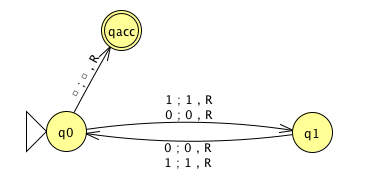
\includegraphics[width=2in]{../../resources/machines/Week8WarmupTM1.png} 

\columnbreak

$M_2$ 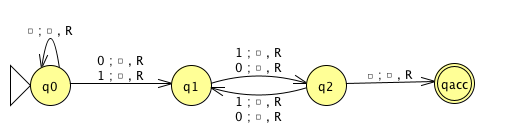
\includegraphics[width=2in]{../../resources/machines/Week8WarmupTM2.png}

\columnbreak

$M_3$ 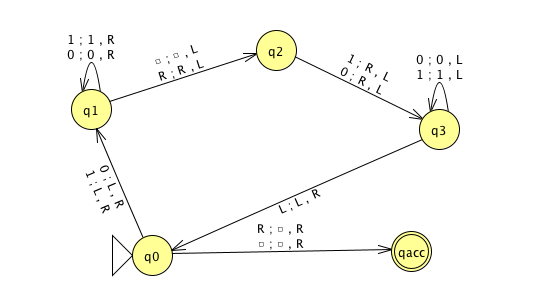
\includegraphics[width=2in]{../../resources/machines/Week8WarmupTM3.png}
\end{multicols}

Example strings in $A_{TM}$

\vfill

Example strings in  $E_{TM}$

\vfill

Example strings in  $EQ_{TM}$

\vfill

\newpage

{\bf  Theorem}: $A_{TM}$  is  Turing-recognizable.


{\bf  Strategy}:  To prove this theorem, we need  to  define  a Turing  machine  $R_{ATM}$ such that 
$L(R_{ATM}) = A_{TM}$.


Define $R_{ATM} =  $ ``

\vspace{150pt}


Proof of correctness: 


\vfill
\vfill

We will show that $A_{TM}$ is undecidable.   {\it First, let's explore what that means.}

\newpage

A {\bf Turing-recognizable} language is a set of strings that 
is the language recognized by some Turing machine. We also 
say that such languages are recognizable.

A {\bf Turing-decidable} language is a set of strings that 
is the language recognized by some decider. We also 
say that such languages are decidable.

An {\bf unrecognizable} language is a language that is not Turing-recognizable.

An {\bf undecidable} language is a language that is not Turing-decidable.


{\bf  True} or {\bf False}: Any  undecidable language  is  also  unrecognizable.


{\bf  True} or {\bf False}: Any  unrecognizable language  is  also  undecidable.


To prove that a computational problem is {\bf decidable}, we find/ build a Turing 
machine that recognizes the language encoding the computational problem, and that 
is a decider.


How do we prove a specific problem is {\bf not decidable}?

How would we even find such a computational problem?


{\it Counting arguments for the existence of an undecidable language:}
\begin{itemize}
    \item The set of all Turing machines is countably infinite.
    \item Each Turing-recognizable language is associated with a Turing machine
    in a one-to-one relationship, so there can be no more Turing-recognizable
    languages than there are Turing machines. 
    \item Since there are infinitely many Turing-recognizable languages
    (think of the singleton sets), there are countably infinitely 
    many Turing-recognizable languages.
    \item Such the set of Turing-decidable languages is an infinite subset 
    of the set of Turing-recognizable languages, the set of 
    Turing-decidable languages is also countably infinite.
\end{itemize}

Since there are uncountably many languages (because $\mathcal{P}(\Sigma^*)$
is uncountable), there are uncountably many unrecognizable languages
and there are uncountably many undecidable languages.


Thus, there's at least one undecidable language!

\vfill

{\bf What's a specific example of a language that is unrecognizable or undecidable?}

To prove that a language is undecidable, we need to prove that there is no Turing machine that decides it.

{\bf Key idea}: proof by contradiction relying on self-referential disagreement.

